\begin{figure}[p]
  \centering
  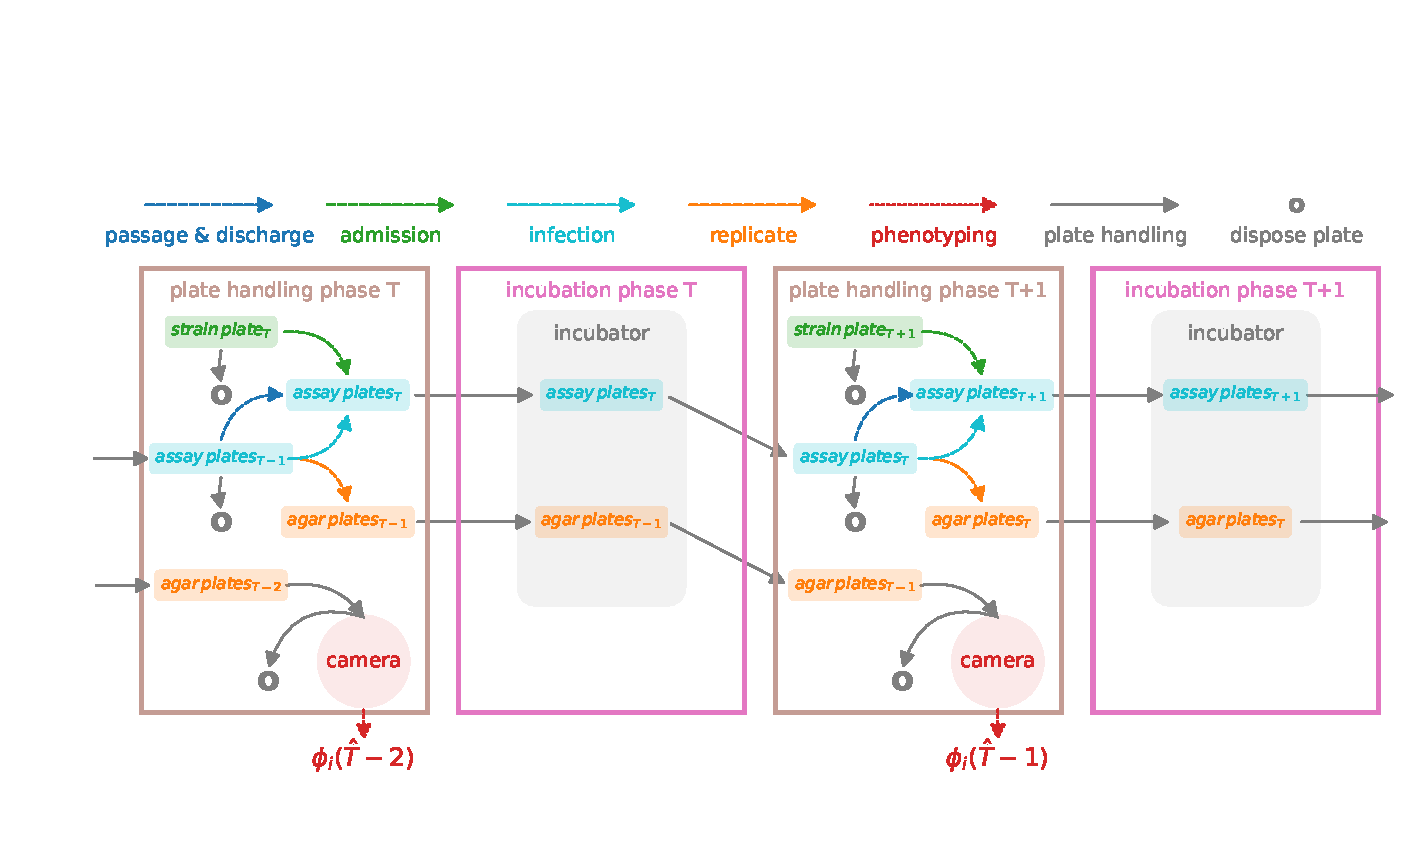
\includegraphics[width = \linewidth]{chapter_2_sup/figures/setup.pdf}
  \caption{
    Schematic illustrating the procedure used in the experiment for transfers T and T+1  in the liquid handling platform after adding medium and drugs to the \textit{assay plates}.
    Every transfer (day), we provide new  \textit{assay} and \textit{agar plates}.
    Plates from the previous transfers are removed.
    To inoculate the new \textit{assay plates} with newly admitted patients from the strain plate, along with staying patients and infection between patients from the previous \textit{assay plate}, we use a pintool with retractable pins (dashed lines).
    Discharged patients are not transferred (pins retracted) to the new assay plates.
  Plates are then automatically transferred (solid lines) to the incubator for overnight incubation. Subsequently, we replicate each \textit{assay plate} onto four agar plates using the pintool. These plates are treated with antibiotics A, B, and AB, and one remains untreated. Once the agar plates have been incubated overnight, we capture images (dotted lines) to determine the resistance profile $\phi_i$ for each well $i$.}
  \label{fig:procedure}
\end{figure}

\begin{figure}[p]
  \vspace{5cm}
  \centering
  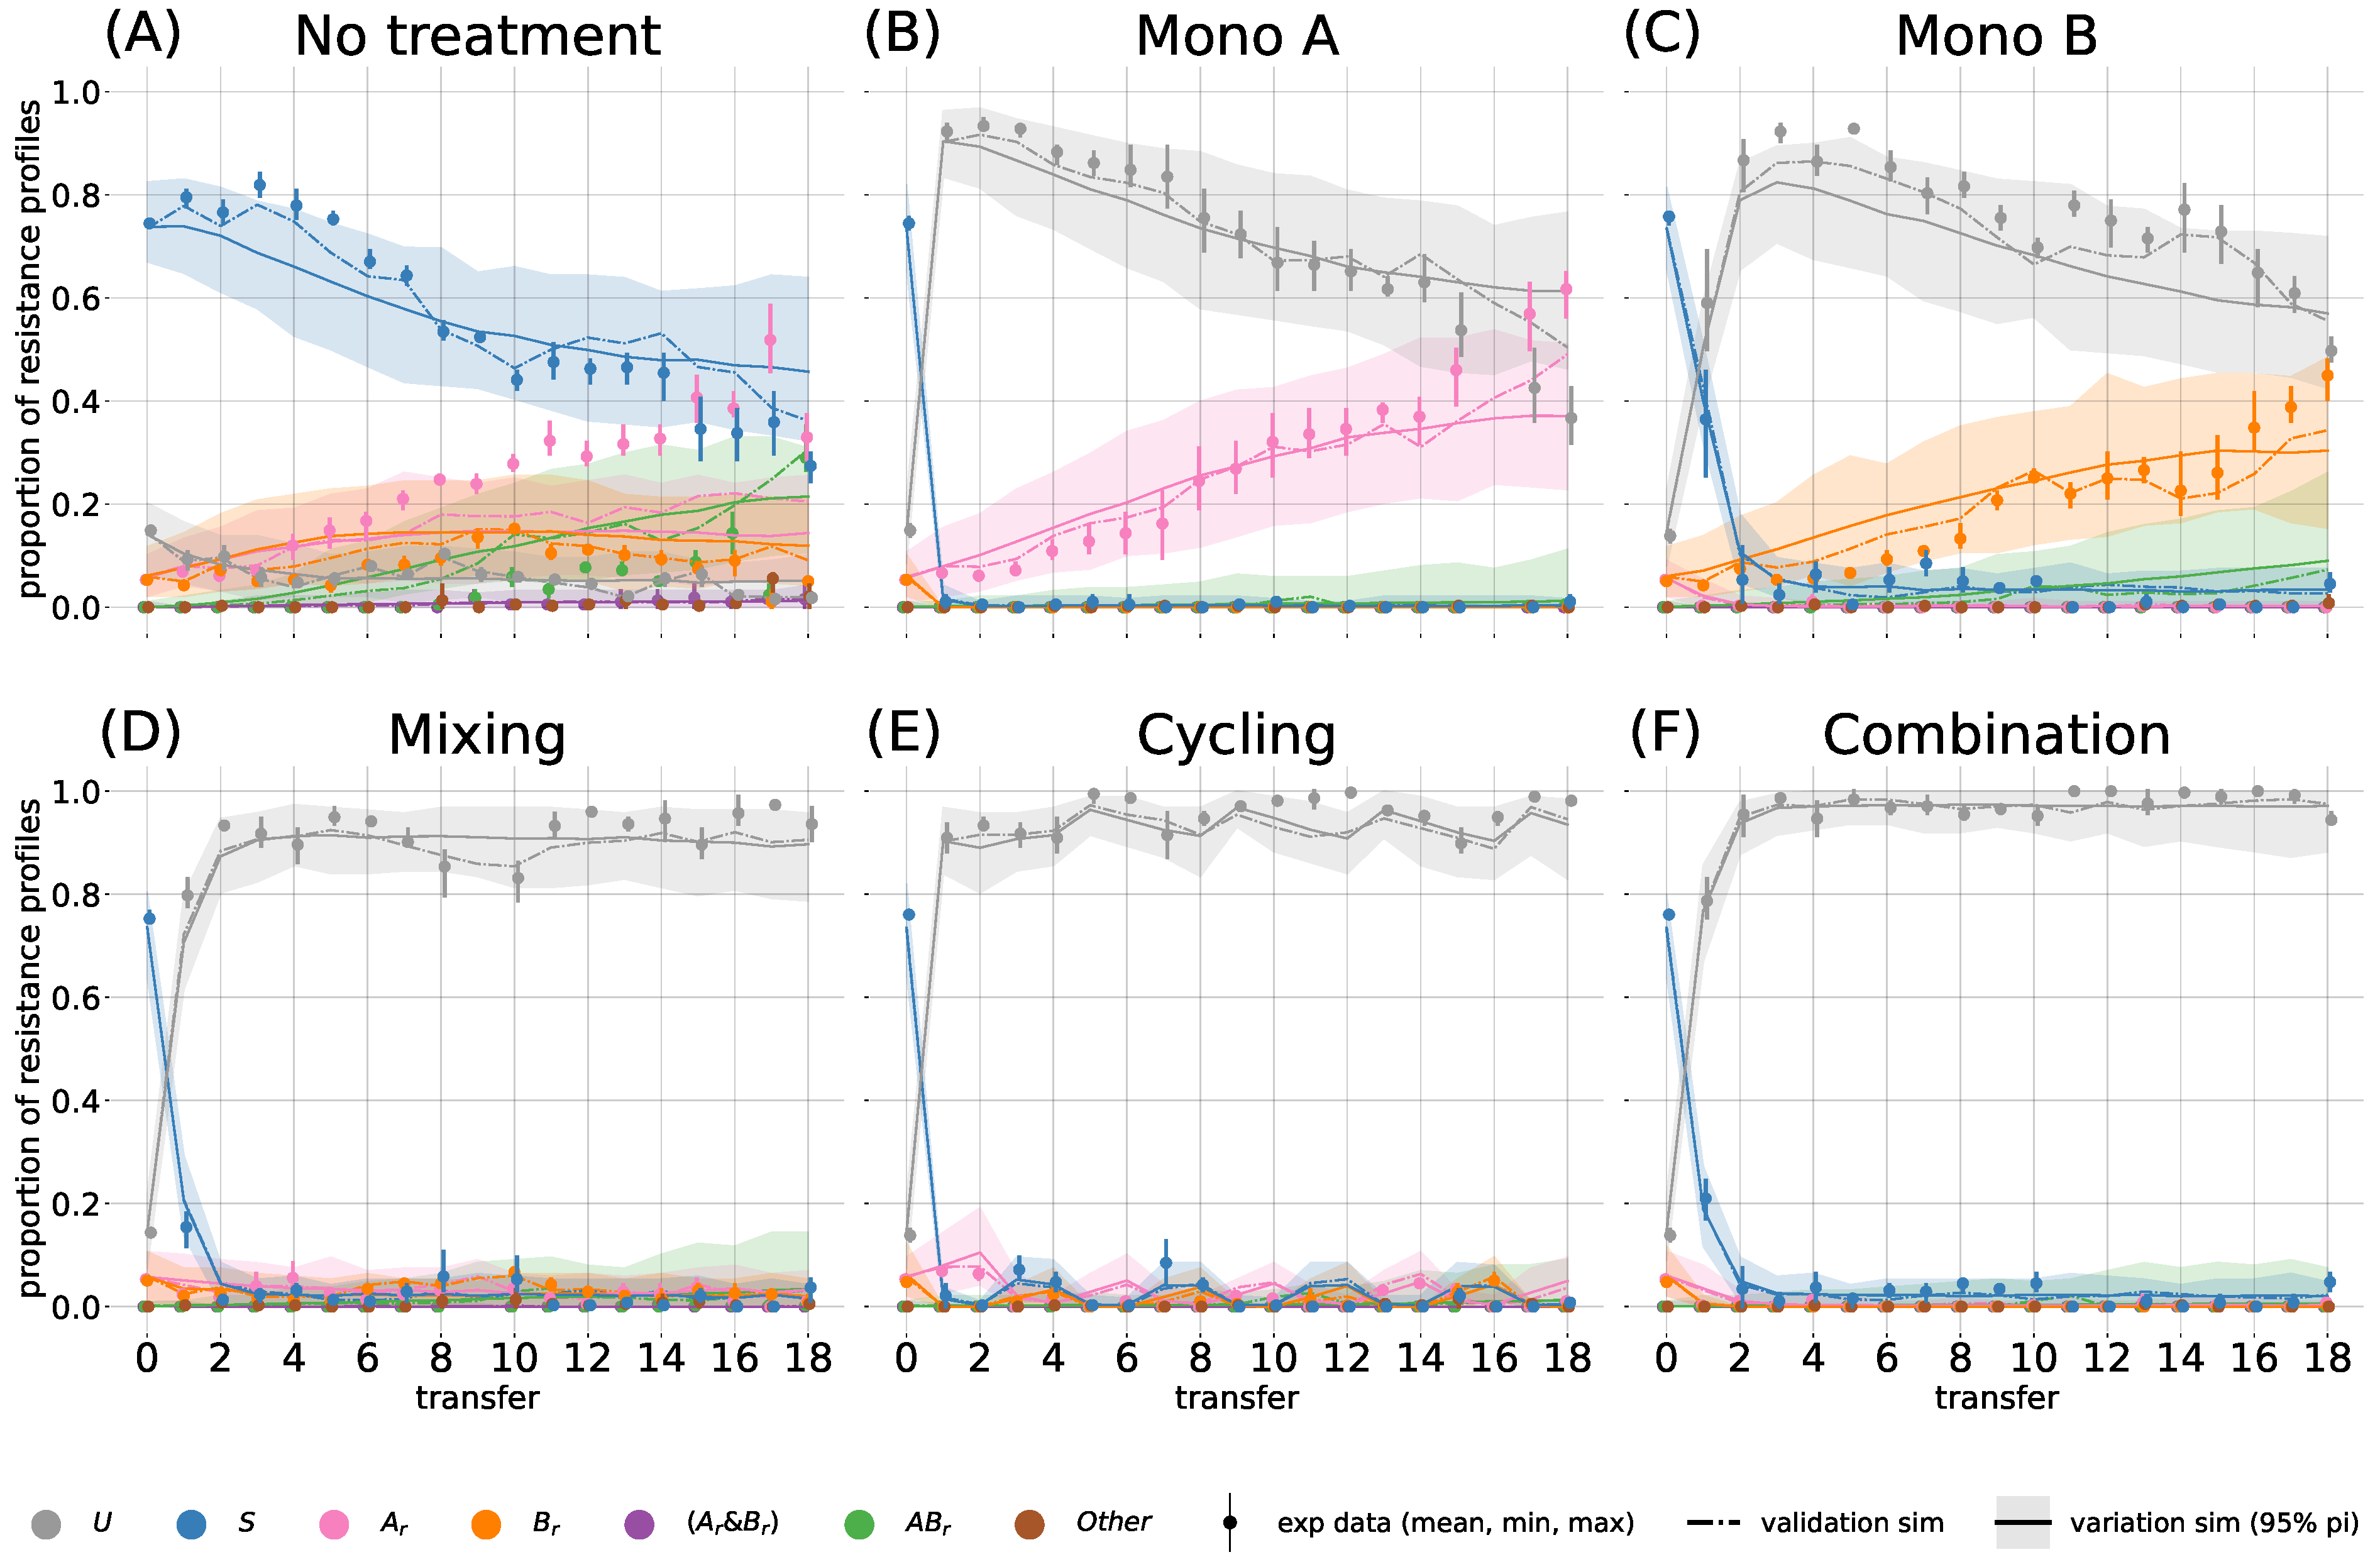
\includegraphics[width=\linewidth]{chapter_2_sup/figures/20210417_timeplot.pdf}
  \caption{\textbf{\textit{Prevention}~scenario:}
    Frequencies of resistance profiles (colours) over time during the \textit{prevention}~scenario.
    The dots show the experimental measurements, and the error bar indicates the min/max interval between the replicates.
    The dash-dotted line shows the mean value of 100 stochastic simulations based on the instruction set used in the in vitro experiment.
    The solid line represents the mean value of 100 simulations with randomly created instruction sets based on the parameter set used in the experiment.
  The shaded error band indicates the 95-percentile interval between the simulations.}
  \label{fig:exp1}
\end{figure}

\begin{figure}[p]
  \centering
  \tikzpanel[0pt]{0.48\linewidth}{chapter_2_sup/tikz/stoch_exp.tex}{}{fig:stoch_exp}
  \tikzpanel[0pt]{0.48\linewidth}{chapter_2_sup/tikz/stoch_val.tex}{}{fig:stoch_val}
  \tikzpanel[0pt]{0.48\linewidth}{chapter_2_sup/tikz/stoch_var.tex}{}{fig:stoch_var}
  \tikzpanel[0pt]{0.48\linewidth}{chapter_2_sup/tikz/stoch_par.tex}{}{fig:stoch_par}
  \caption{Illustration depicting the various sources of stochasticity and variation in experiments and simulations.
    Our experiments and simulations investigate various sources of stochasticity and their contributions to the variability of the outcome. In panels \textbf{A}-\textbf{D}, we sketch the different sources of stochasticity for each experiment and simulation, highlighting our primary focus in red.
    \textbf{(A) \textit{In vitro} Experiment.} Each experiment explores a scenario and is defined by a distinct parameter set (\textit{prevention} (P), \textit{containment} (C), \textit{maximum emergence} (E)). We randomly generated one instruction set for each parameter set~$i$: \ensuremath{{}^{i}\!z^{1}}. For each instruction set \ensuremath{{}^{i}\!z^{1}}, we replicated the cumulative in-well dynamics four times \ensuremath{{}^{i}\!r^{1}_{j}}.
    \textbf{(B) Validation Simulation.} To assess our computational model, we employed identical parameter sets and instruction sets \ensuremath{{}^{i}\!z^{1}}, as employed in the \textit{in vitro} experiments. For each instruction set \ensuremath{{}^{i}\!z^{1}}, we conducted 100 stochastic simulations \ensuremath{{}^{i}\!s^{1}_{j}}.
    \textbf{(C) Variation Simulation.} For every \textit{in vitro} parameter set, we randomly generated 100 alternative instruction sets \ensuremath{{}^{i}\!z^{k}} to quantify the influence of experimental decisions on the experiment's outcomes. For each instruction set, we performed one simulation \ensuremath{{}^{i}\!s^{k}_{1}}.
    \textbf{(D) \textit{In Silico} Sensitivity Analysis.}
  We examined the sensitivity of our experimental findings to the input parameters by examining the effects of varying the input parameters on the resulting frequency of uninfected cases for different treatment strategies. To achieve this, we generated 20{,}000 alternative parameter sets \ensuremath{{}^{i}\!p}. We created ten randomised instruction sets \ensuremath{{}^{i}\!z^{k}} for each parameter set~\ensuremath{{}^{i}\!p} and simulated each instruction set one time (\ensuremath{{}^{i}\!s^{k}_{1}}).}
  \label{fig:stochs}
\end{figure}

\begin{figure}[p]
  \centering
  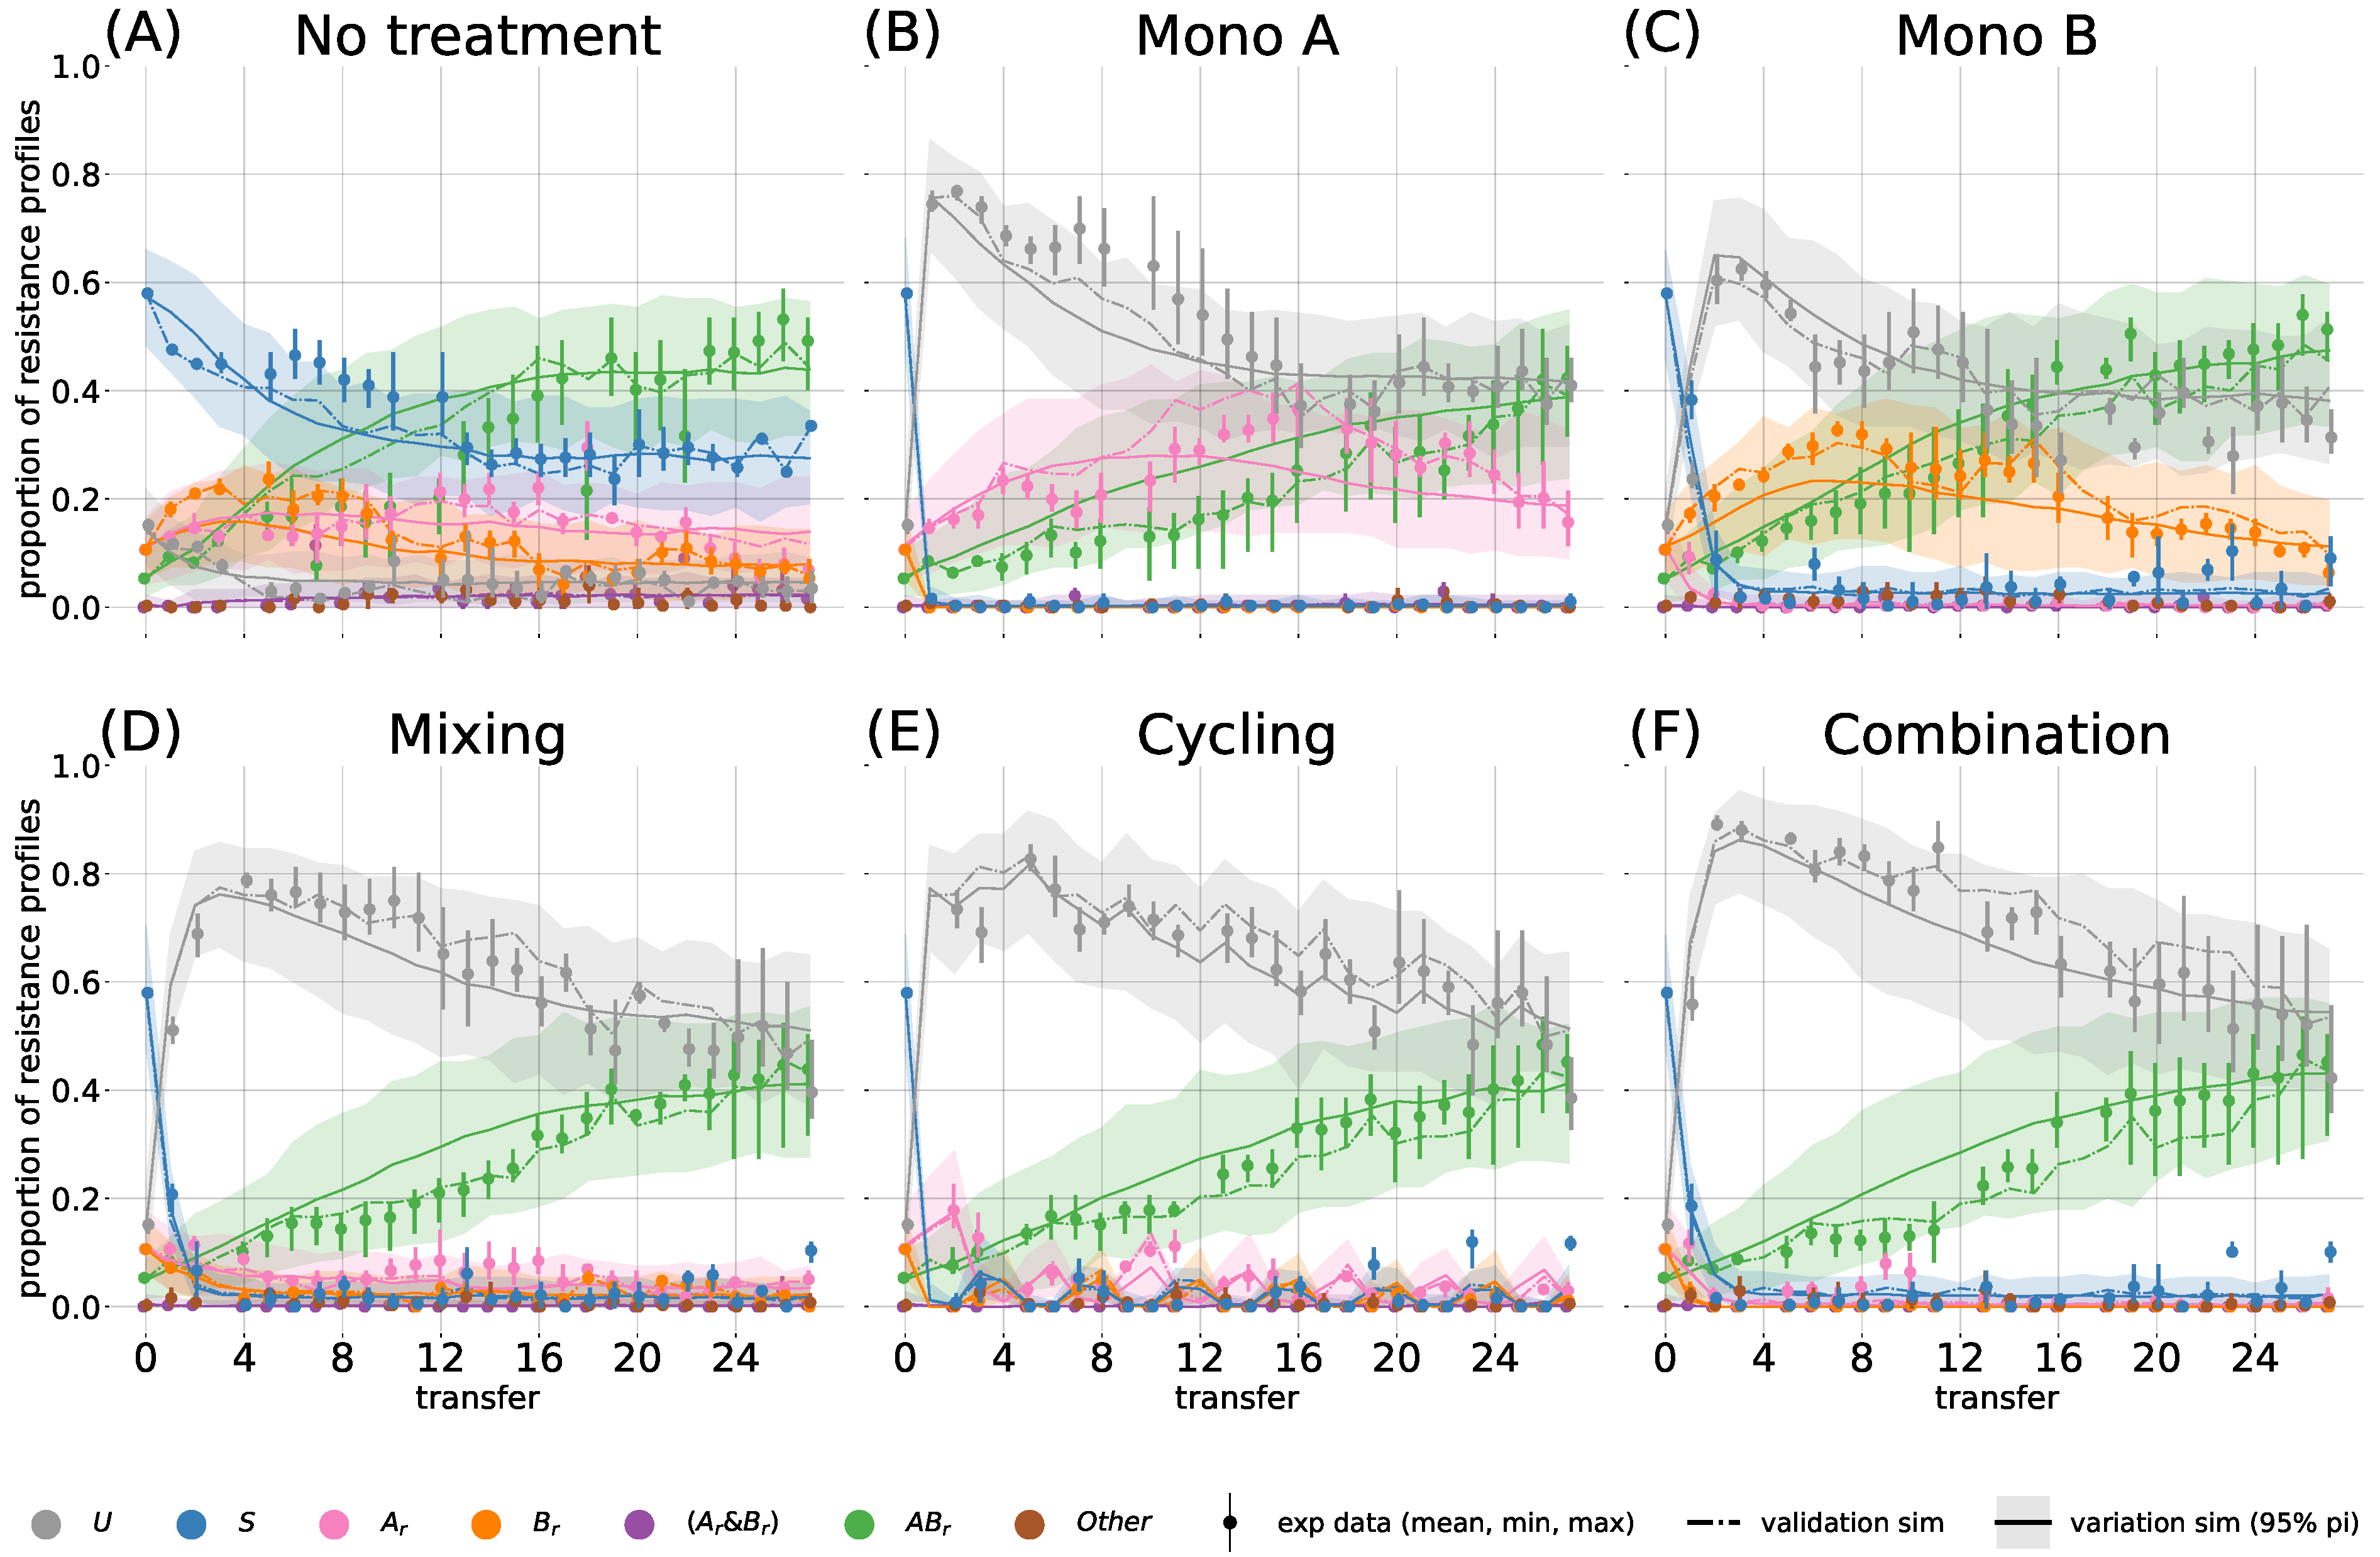
\includegraphics[width = \linewidth]{chapter_2_sup/figures/20220127_timeplot.pdf}
  \caption{\textbf{\textit{Containment} scenario:}
    Frequencies of resistance profiles (colours) over time during the \textit{containment}~scenario.
    The dots show the experimental measurements, and the error bar indicates the min/max interval between the replicates.
    The dash-dotted line shows the mean value of 100 stochastic simulations based on the instruction set used in the in vitro experiment.
    The solid line represents the mean value of 100 simulations with randomly created instruction sets based on the parameter set used in the experiment.
  The shaded error band indicates the 95-percentile interval between the simulations.}
  \label{fig:exp2}
\end{figure}

\clearpage
\begin{figure}[p]
  \subpanel[xshift = -10pt]{.6\linewidth}{
    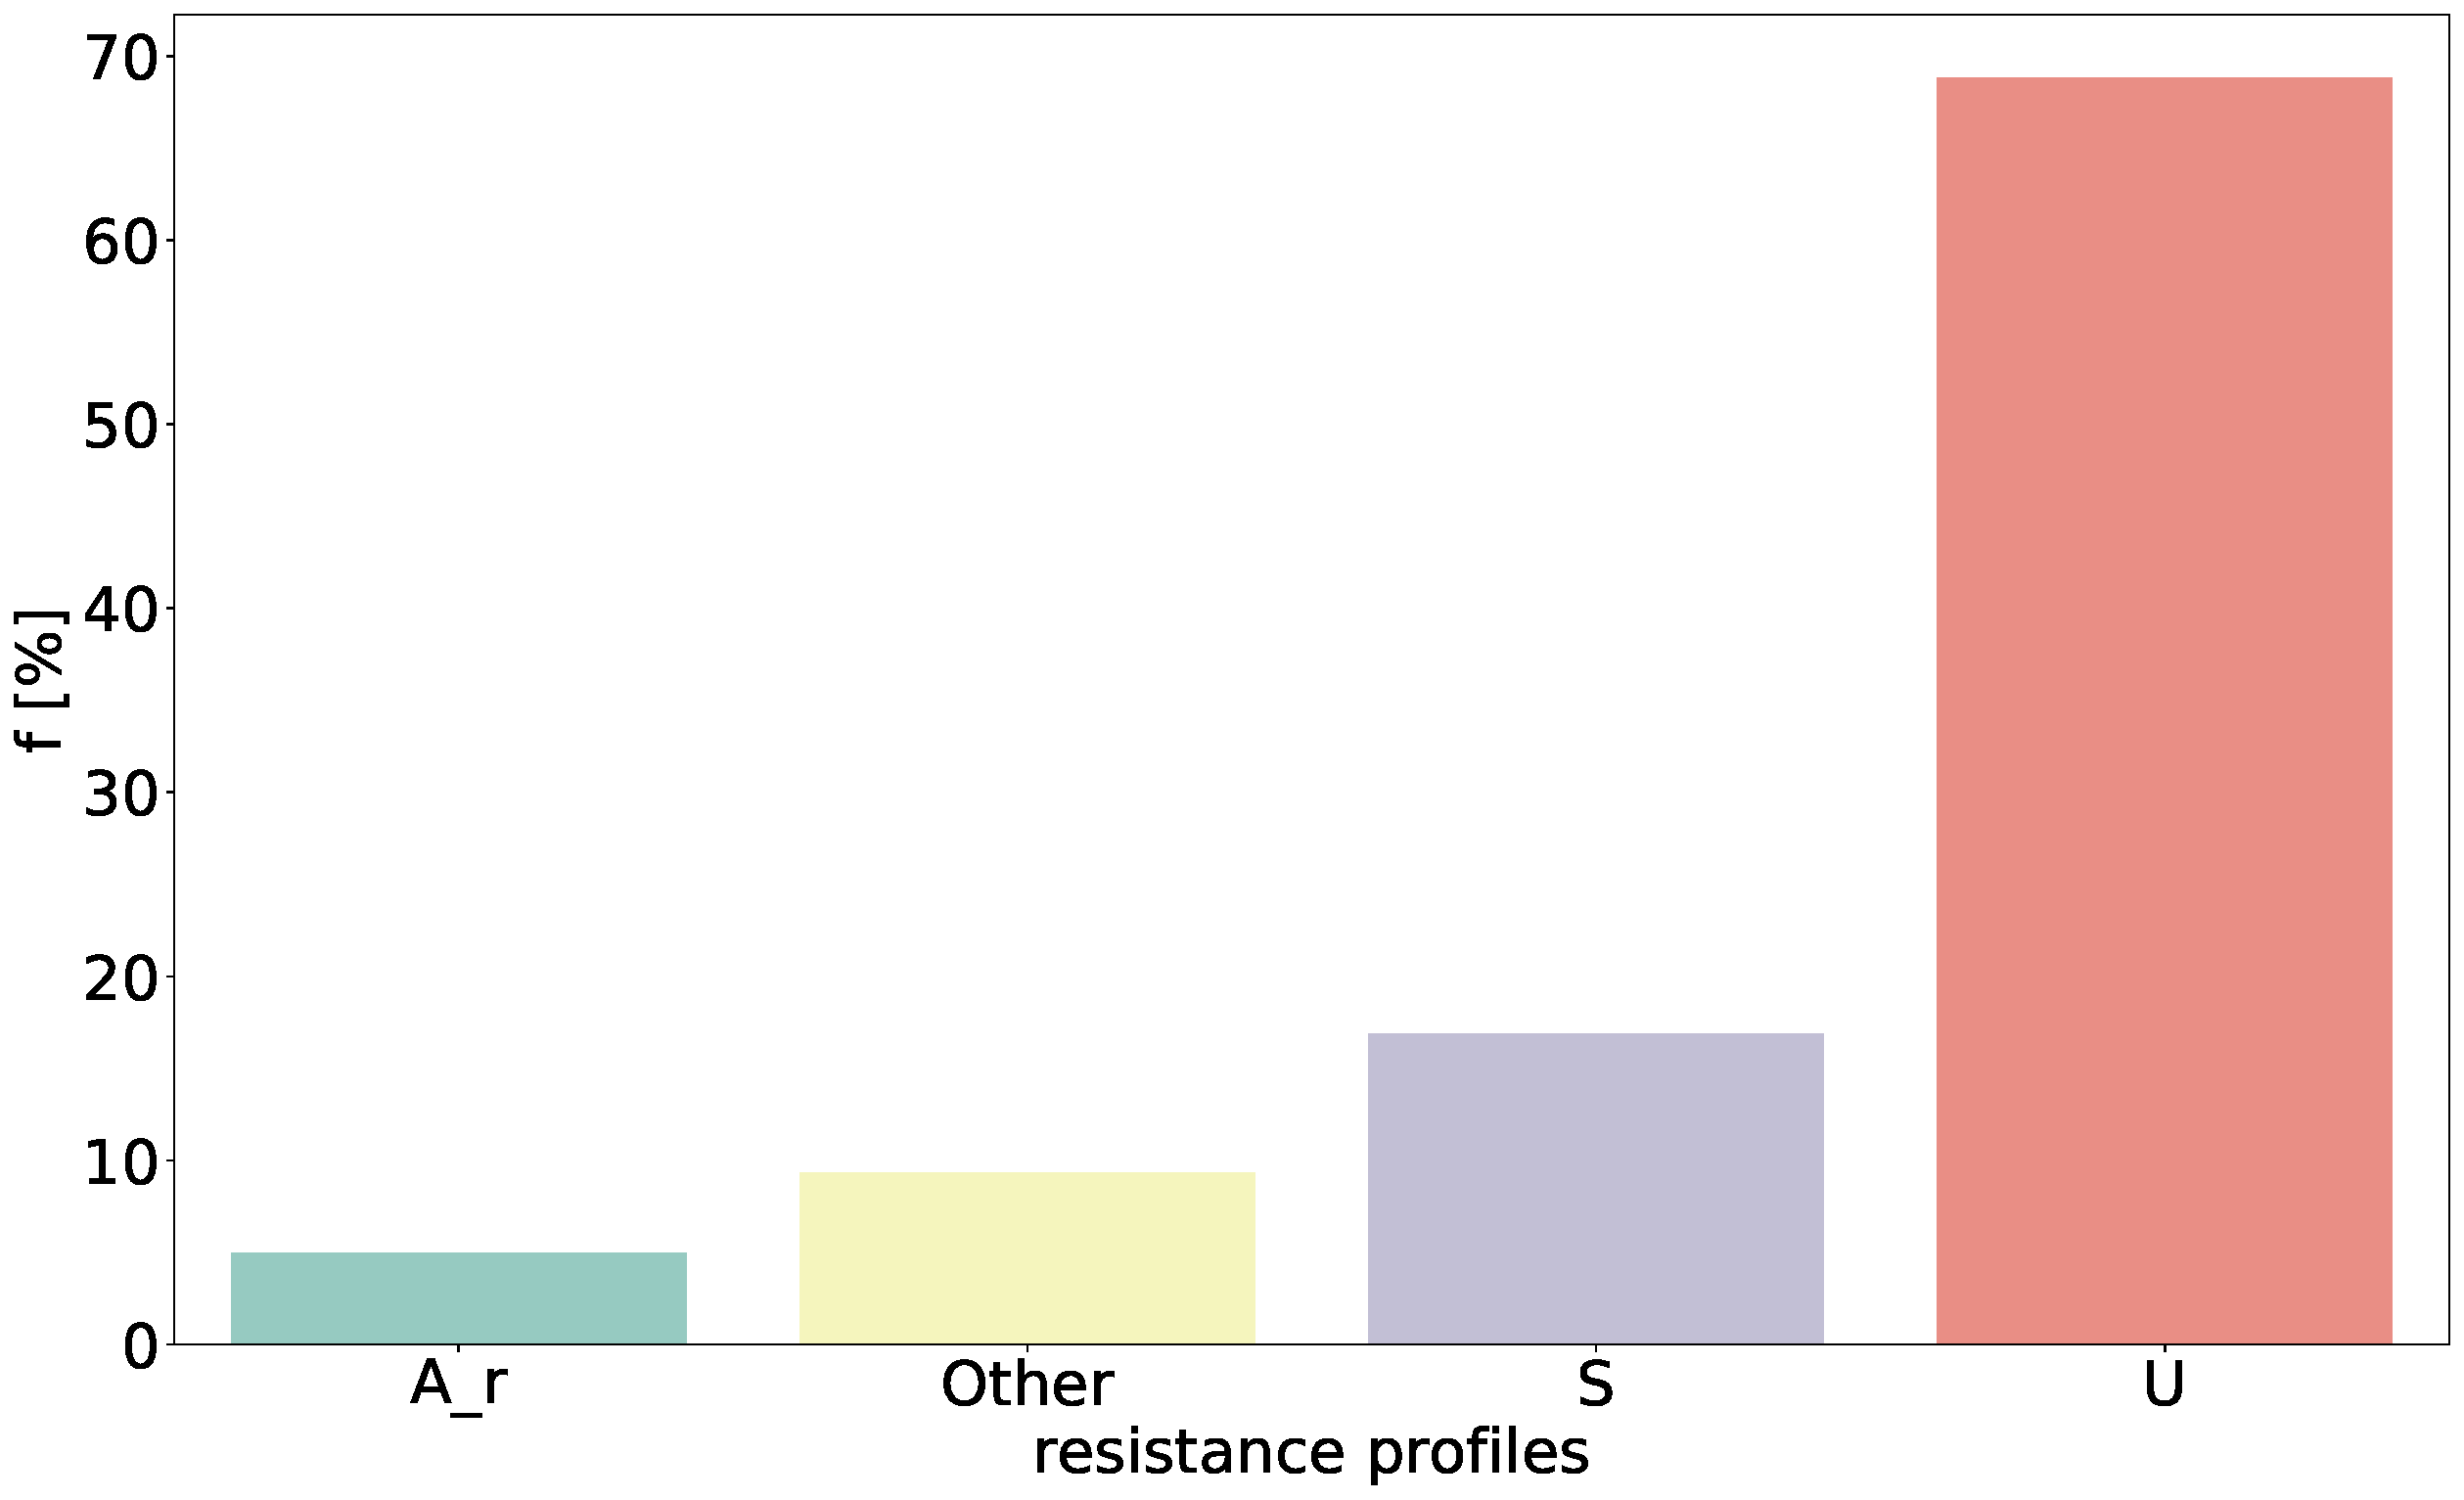
\includegraphics[width=\linewidth]{chapter_2_sup/figures/20220412_Ar_resulting_phenotypes.pdf}
  }{}{fig:BtreatAr}
  \hfill
  \tikzpanel[0pt]{.4\linewidth}{chapter_2_sup/tikz/phenotyping.tex}{}{fig:phenotyping}
  \caption{
    \textbf{(A)}
    Experimentally measured resistance profiles for 1784 wells with the pre-treatment profile \( A_r \) and treatment with drug B during the \textit{maximum-emergence}~scenario.
    \textbf{(B)}
    Decision tree to calculate the distribution of measured phenotypes for a well that contains \( Z_\emptyset \) sensitive and \( Z_A \) A-resistant bacteria.
    $g_\vartheta$ is the probability of drawing a drop that forms a colony on a plate treated with drug $\vartheta$, while $g_\vartheta'$ is the probability that it does not form a colony.
  }
\end{figure}

\clearpage
\begin{figure}
  \centering
  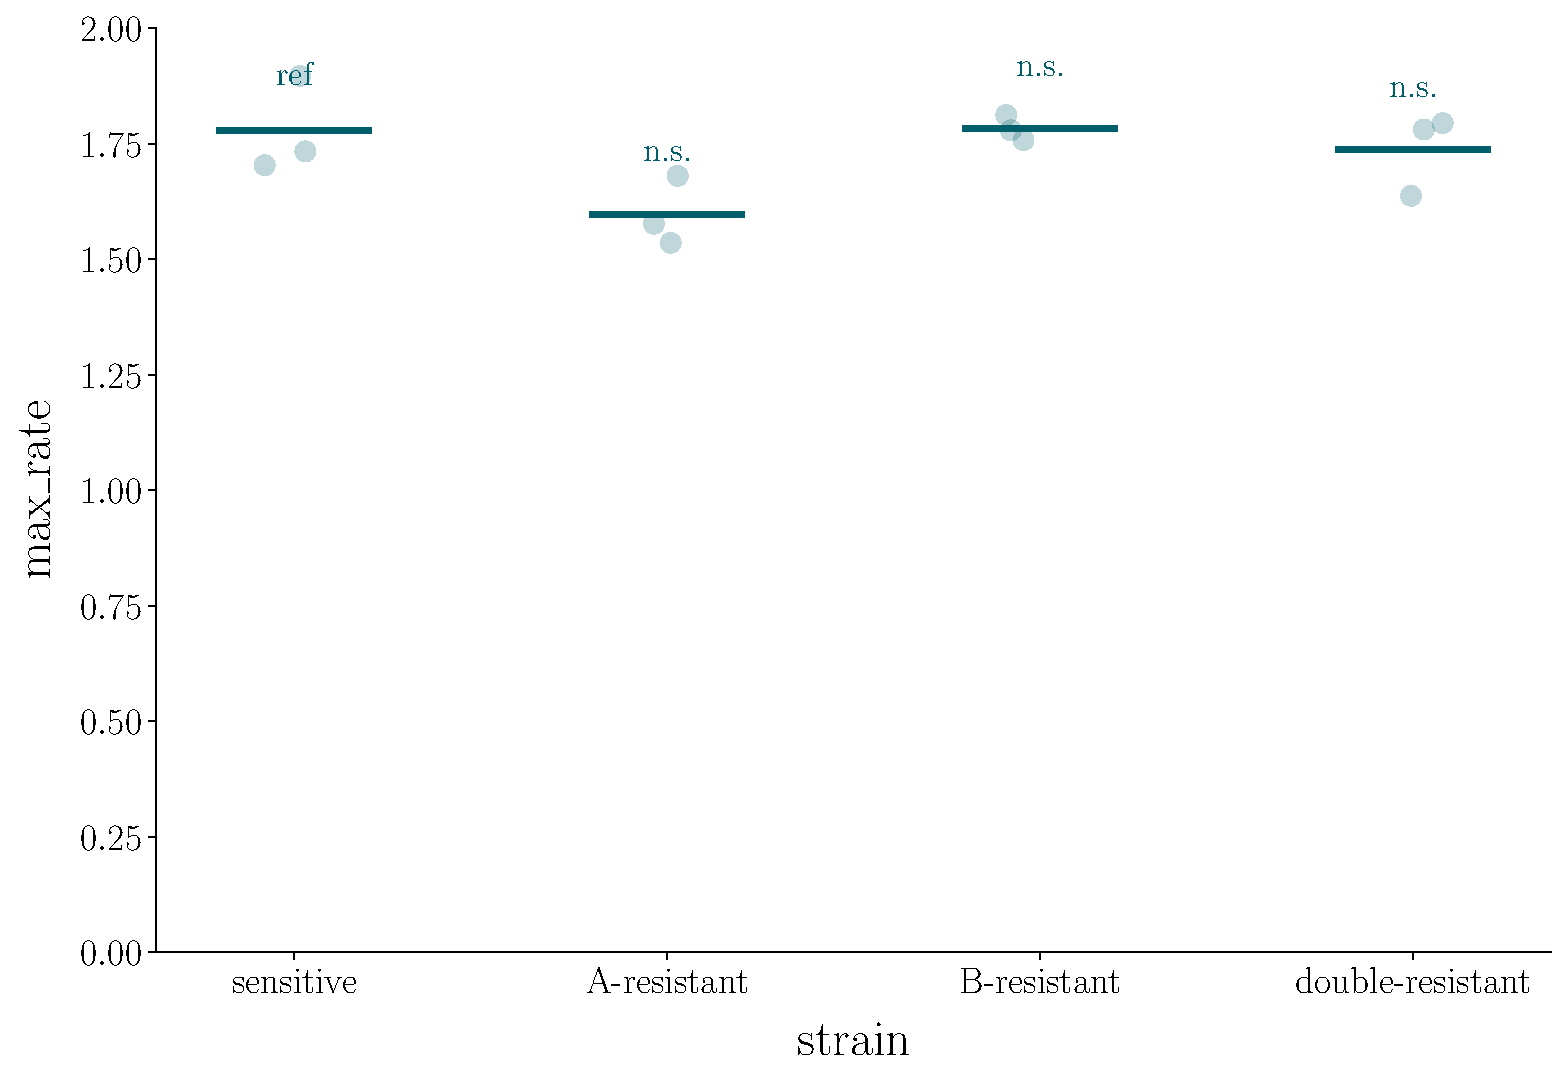
\includegraphics[width=\linewidth]{chapter_2_sup/figures/plasmid_costs.pdf}
  \caption{
    Maximum growth rates of sensitive and plasmid-carrying strains, measured using OD-growth curves.
    Each dot represents an individual well, and vertical bars indicate the mean.
    The sensitive strain was used as the reference ("ref") for pairwise comparisons to the plasmid-carrying strains to identify potential plasmid costs.
    We used the Mann-Whitney U tests with the Bonferroni correction to identify significant differences in growth rates. All pairwise comparisons were not significant (n.s.).
  }
  \label{fig:plasmid_costs}
\end{figure}

\clearpage
\begin{figure}[p]
  \centering
  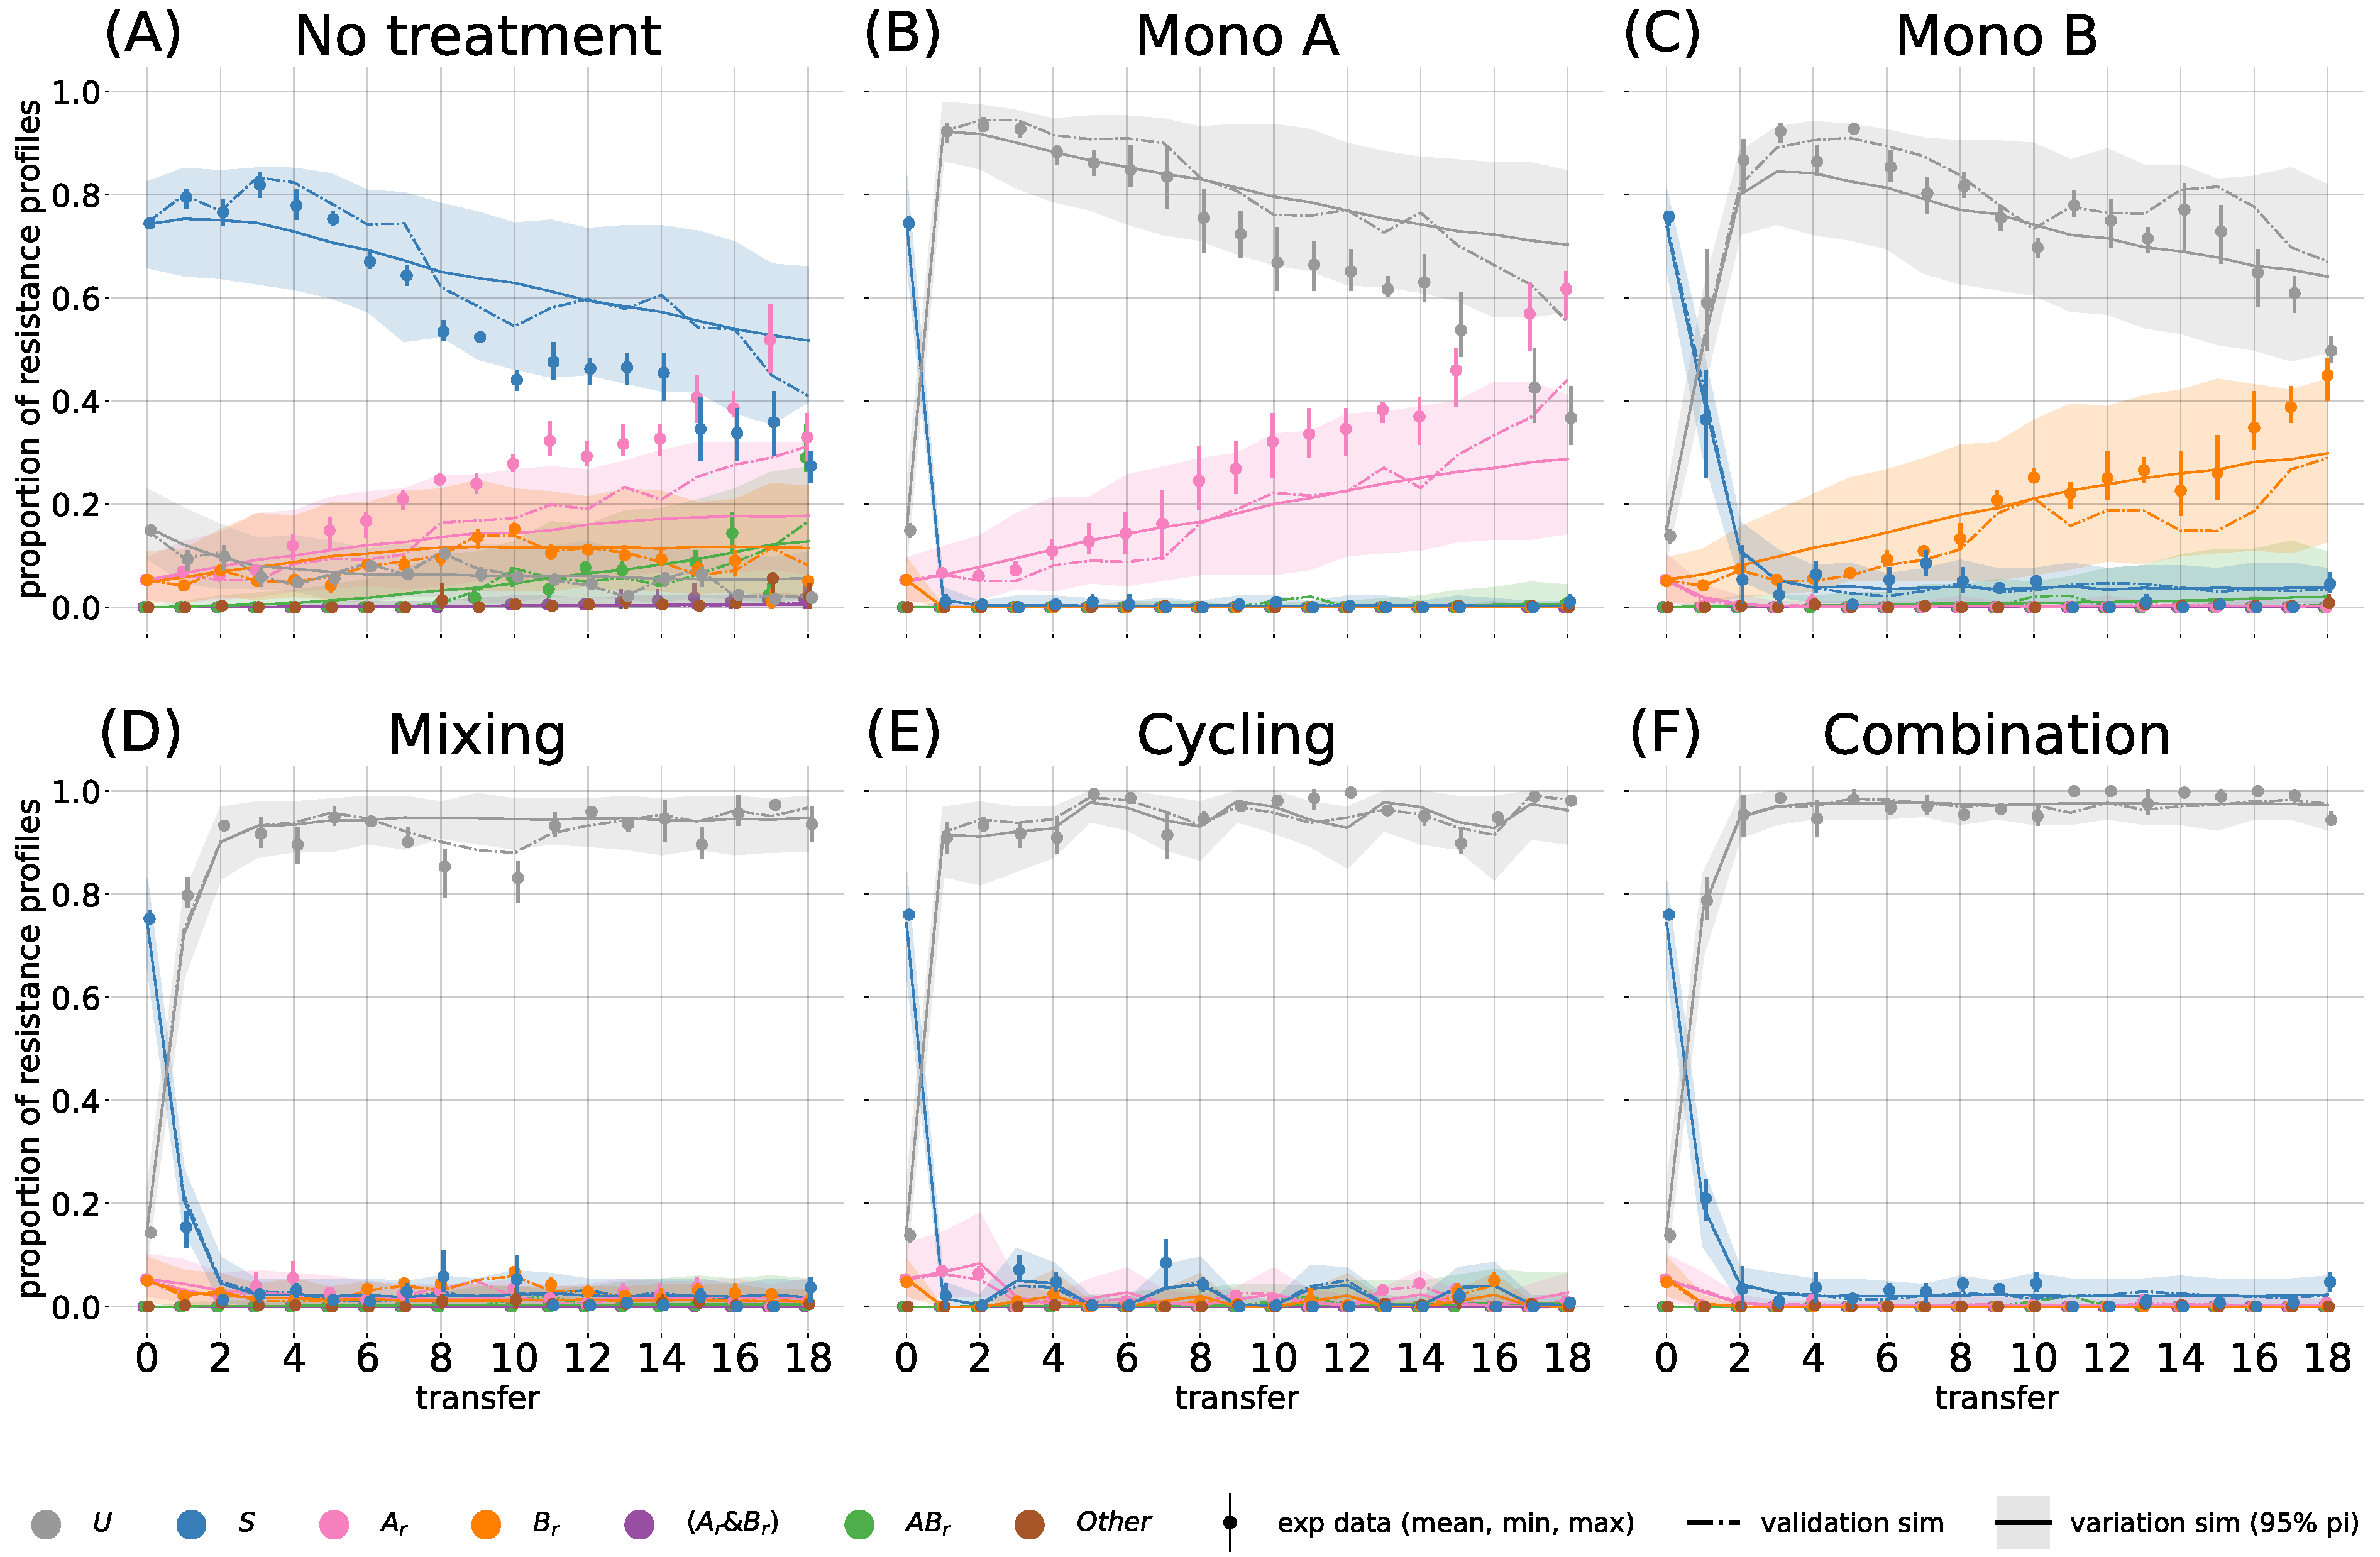
\includegraphics[width=\linewidth]{chapter_2_sup/figures/20210417_timeplot_clean.pdf}
  \caption{\textbf{\textit{Prevention}~scenario with filtered transition probabilities.}
    Frequencies of resistance profiles (colours) over time during the \textit{prevention} scenario.
    The dots show the experimental measurements, and the error bar indicates the min/max interval between the replicates.
    The dash-dotted line shows the mean value of 100 stochastic simulations based on the instruction set used in the in vitro experiment.
    The solid line represents the mean value of 100 simulations with randomly created instruction sets based on the parameter set used in the experiment.
  The shaded error band indicates the 95-percentile interval between the simulations.}
  \label{fig:exp1_filtered}
\end{figure}

\begin{figure}[p]
  \centering

  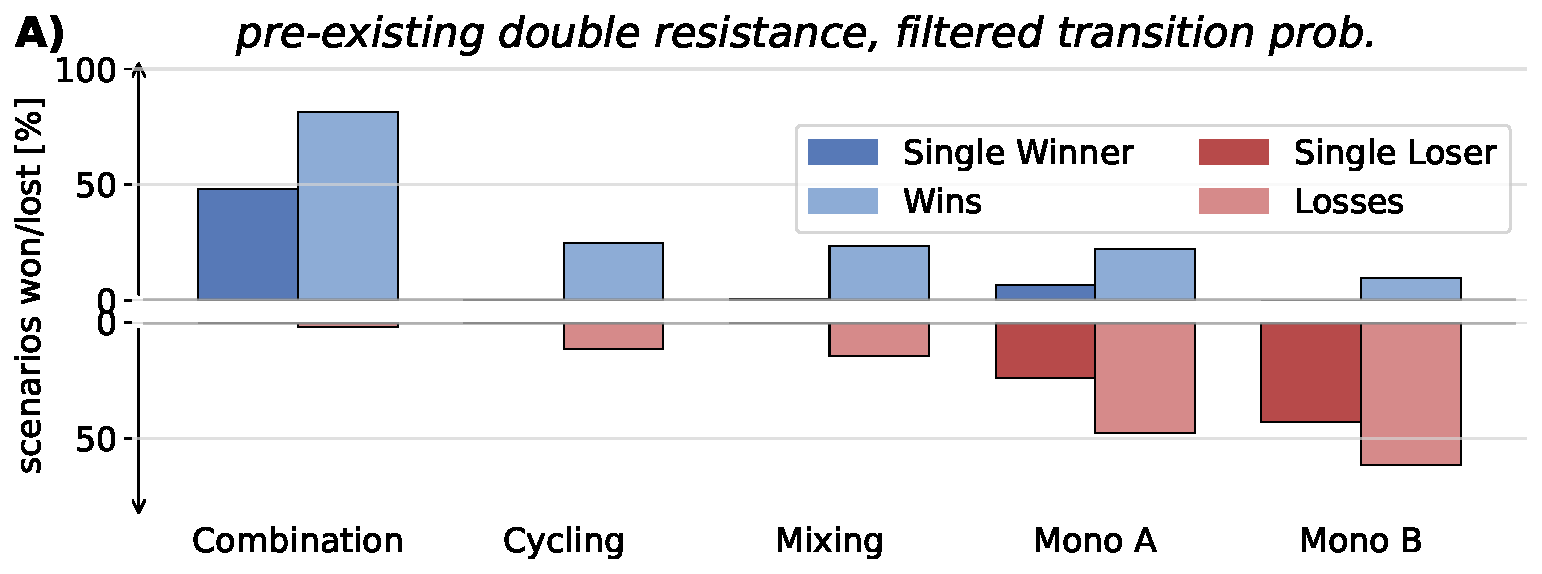
\includegraphics[width = \linewidth]{chapter_2_sup/figures/wins_and_losses_clean_preexisting.pdf}
  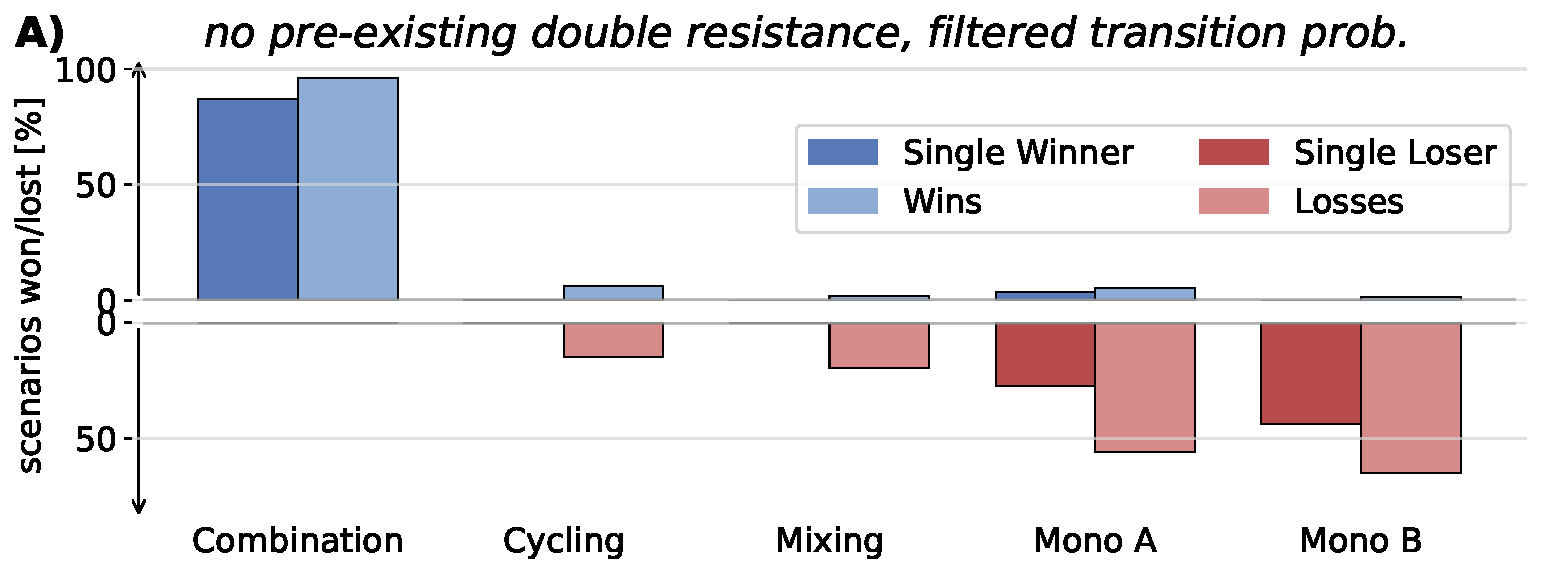
\includegraphics[width = \linewidth]{chapter_2_sup/figures/wins_and_losses_clean_no_preex.pdf}
  \caption{
    Sensitivity analysis using filtered transition probabilities.
    We evaluated the effectiveness of the five treatment strategies in maximising the frequency of uninfected \textit{in silico} patients across randomly generated parameter sets.
    Strategies not significantly better than any other are marked as losers (pastel red), with those significantly worse than all others being labelled as single losers (dark red).
    Conversely, strategies that are not significantly worse than any other are classified as winners (pastel blue), and those significantly better than all others as single winners (dark blue).
    \textbf{(A)} Evaluation of 10,000 parameter sets with preexisting double resistance. 659 out of 10,000 parameter sets yielded no significant difference between the strategies.
    \textbf{(B)} Evaluation of 10,000 parameter sets without preexisting double resistance. 8 out of 10,000 parameter sets yielded no significant difference between the strategies.
  }
  \label{fig:senstivity_clean}
\end{figure}
